\begin{frame}{Main math results: \PAL{} improves across datasets}
\small
\begin{figure}
\centering
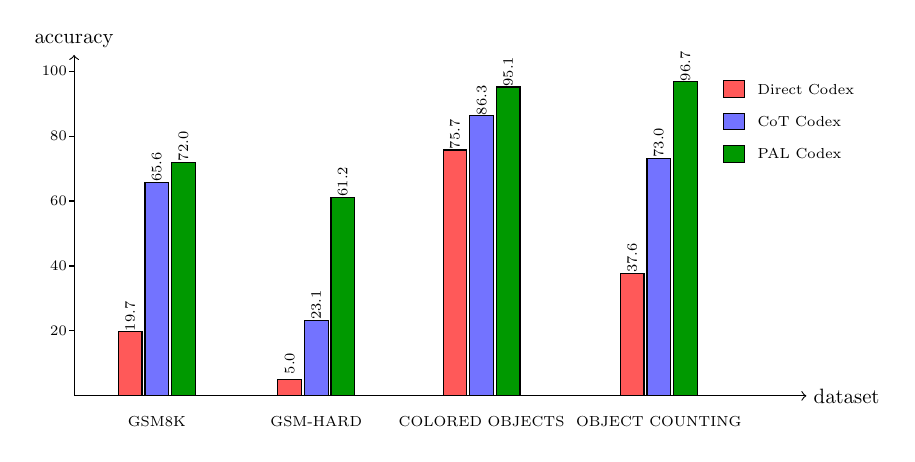
\begin{tikzpicture}[scale=0.75, transform shape, x=1cm, y=0.055cm]

% Axes
\draw[->] (0,0) -- (12.4,0) node[right]{dataset};
\draw[->] (0,0) -- (0,105) node[above]{accuracy};

% Y ticks
\foreach \y in {20,40,60,80,100}
    \draw (-0.08,\y) -- (0,\y)
    node[left]{\scriptsize \y};

% Dataset labels
\node at (1.4,-8) {\scriptsize GSM8K};
\node at (4.1,-8) {\scriptsize GSM-HARD};
\node at (6.9,-8) {\scriptsize COLORED OBJECTS};
\node at (9.9,-8) {\scriptsize OBJECT COUNTING};

% Colors:
% Direct Codex = red
% CoT Codex    = blue
% PAL Codex    = green

% GSM8K
\draw[fill=red!65]          (0.75,0) rectangle (1.15,19.7);
\draw[fill=blue!55]         (1.20,0) rectangle (1.60,65.6);
\draw[fill=green!60!black]  (1.65,0) rectangle (2.05,72.0);

% GSM-HARD
\draw[fill=red!65]          (3.45,0) rectangle (3.85,5.0);
\draw[fill=blue!55]         (3.90,0) rectangle (4.30,23.1);
\draw[fill=green!60!black]  (4.35,0) rectangle (4.75,61.2);

% COLORED OBJECTS
\draw[fill=red!65]          (6.25,0) rectangle (6.65,75.7);
\draw[fill=blue!55]         (6.70,0) rectangle (7.10,86.3);
\draw[fill=green!60!black]  (7.15,0) rectangle (7.55,95.1);

% OBJECT COUNTING
\draw[fill=red!65]          (9.25,0) rectangle (9.65,37.6);
\draw[fill=blue!55]         (9.70,0) rectangle (10.10,73.0);
\draw[fill=green!60!black]  (10.15,0) rectangle (10.55,96.7);

% Value labels
\node[rotate=90] at (0.95,24.5) {\scriptsize 19.7};
\node[rotate=90] at (1.40,70.5) {\scriptsize 65.6};
\node[rotate=90] at (1.85,76.8) {\scriptsize 72.0};

\node[rotate=90] at (3.65,10.0) {\scriptsize 5.0};
\node[rotate=90] at (4.10,28.0) {\scriptsize 23.1};
\node[rotate=90] at (4.55,66.0) {\scriptsize 61.2};

\node[rotate=90] at (6.45,80.5) {\scriptsize 75.7};
\node[rotate=90] at (6.90,91.0) {\scriptsize 86.3};
\node[rotate=90] at (7.35,99.8) {\scriptsize 95.1};

\node[rotate=90] at (9.45,42.5) {\scriptsize 37.6};
\node[rotate=90] at (9.90,78.0) {\scriptsize 73.0};
\node[rotate=90] at (10.35,101.5) {\scriptsize 96.7};

% Legend
\draw[fill=red!65]         (11.0,92) rectangle (11.35,97);
\node[right] at (11.45,94.5) {\scriptsize Direct Codex};

\draw[fill=blue!55]        (11.0,82) rectangle (11.35,87);
\node[right] at (11.45,84.5) {\scriptsize CoT Codex};

\draw[fill=green!60!black] (11.0,72) rectangle (11.35,77);
\node[right] at (11.45,74.5) {\scriptsize PAL Codex};

\end{tikzpicture}
\caption{PAL paper results on arithmetic, symbolic, and algorithmic reasoning benchmarks.}
% \label{fig:pal_selected_results}
\end{figure}
%\begin{block}{Interpretation}
The largest difference appears on \textbf{GSM-HARD}: 
when numbers become large, 
\textbf{CoT} accuracy drops sharply, 
while \textbf{PAL} remains more stable because \textbf{Python performs the arithmetic}.
%\end{block}
\end{frame}
